% !TEX root = ../../thesis.tex

\tikz[remember picture,overlay] \node[inner sep=0pt] at (current page.center){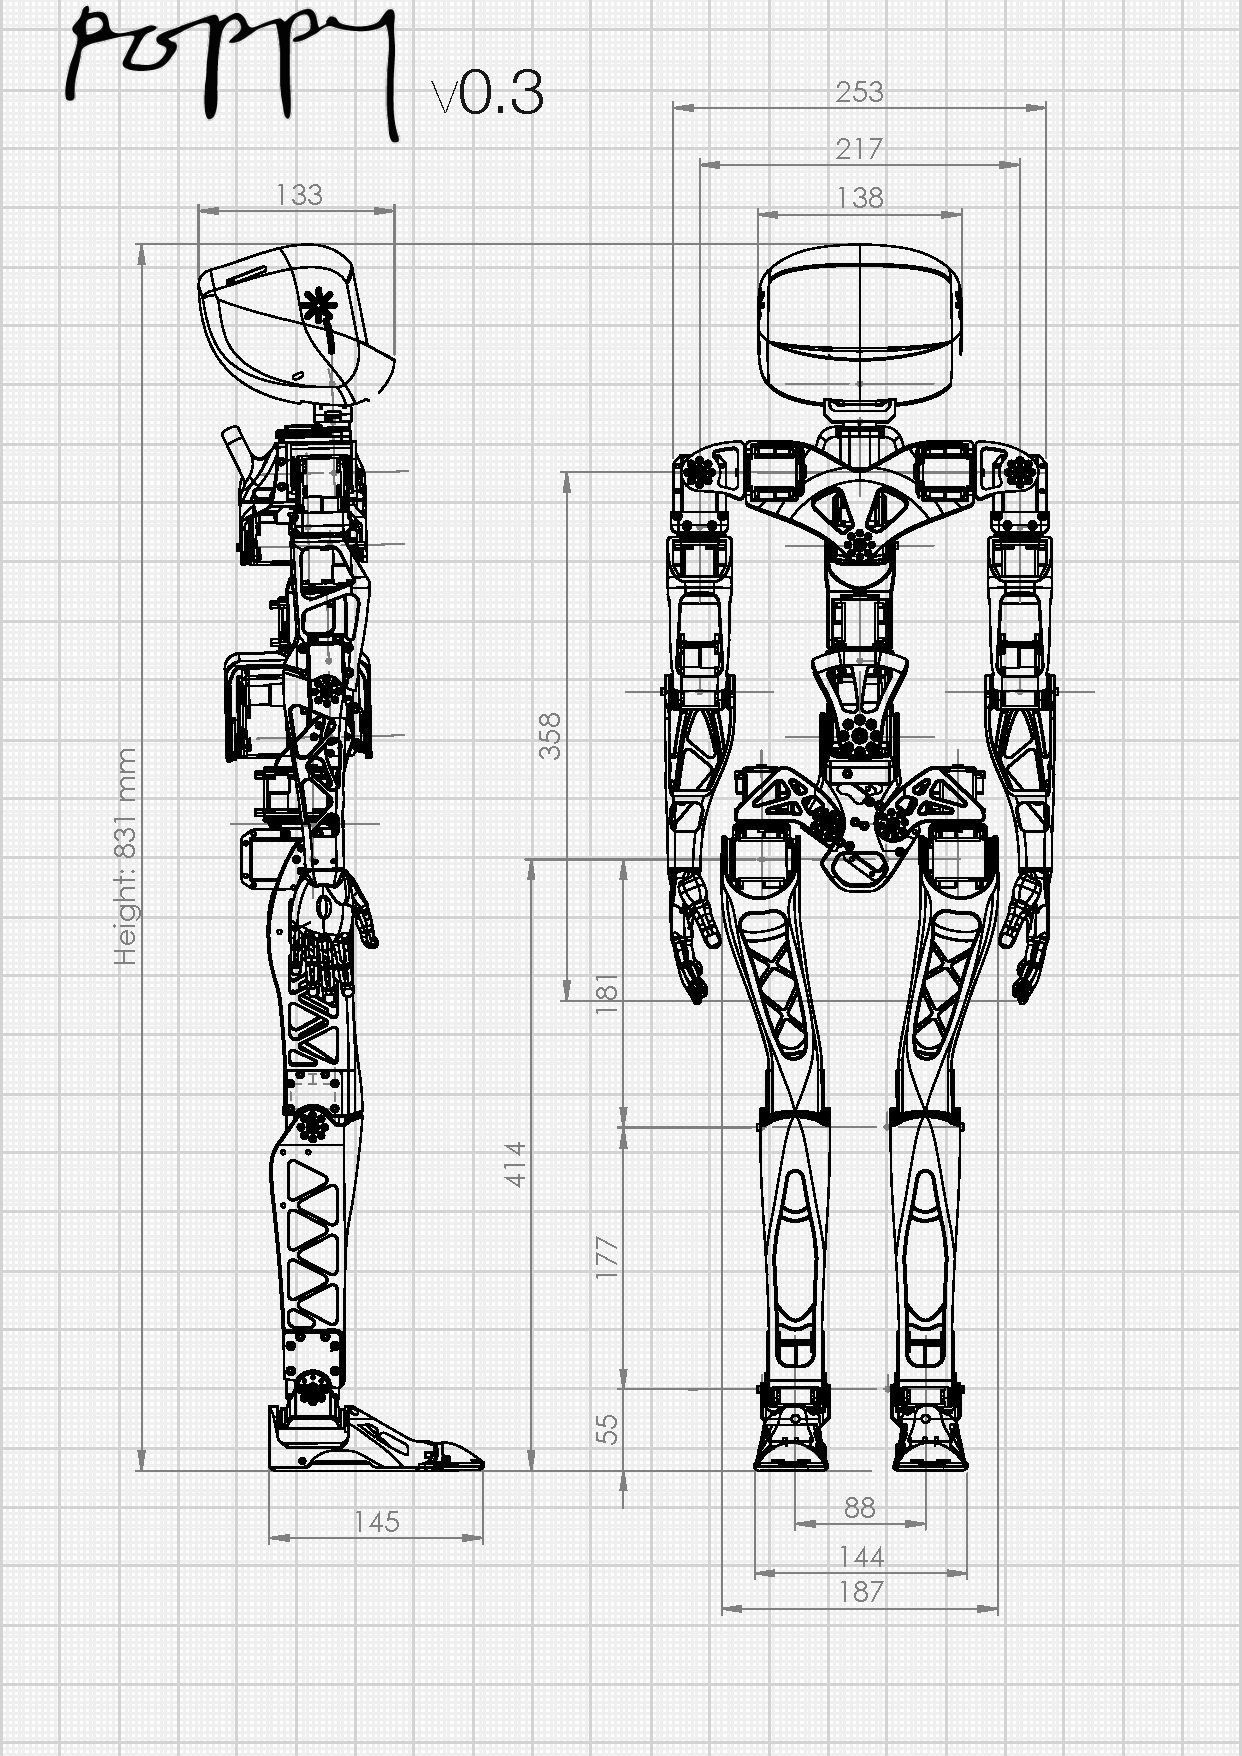
\includegraphics[width=\paperwidth,height=\paperheight]{Poppy_dimensions}};
\clearpage

\section{A little robot} % (fold)

Toward the goals presented in the introduction, the size of the robot is a really important aspect.

On one hand, small size makes very difficult the integration of complex, powerful and accurate mechatronics. Therefore it reduces the scope of technology we could use for the robot. In particular, the integration of hydraulic and pneumatic actuator, as well as advanced mechanisms involving several moving parts is really challenging.

On the other hand, having a small robot is indeed really convenient for exploring morphological properties in the real world.

First, it changes significantly the experimental process: The ratio between weight, and thus energy and torques enforced by movements, and the mechanical robustness of the structure and of the actuators, is such that the robot can fall without breaking itself. Moreover, it is lightweight, which allows people to handle it directly without additional infrastructure and in a secure way. On the one hand, all of this speeds up the experimental process. On the other hand, it changes deeply the methodology of movement and motor skill design by allowing creating movements directly on the robot by real-world experiments without a simulation process. This includes for instance adjusting in real time motor primitives, even extreme ones

Second, this brings advantages regarding human interaction, which is an important focus in this work: On the one hand, from the above reasons, this rules out the problem of physical security in the Human/Robot interaction. On the other hand, the size of the robot plays an important role in the psychological representation that people have of it.

However exploring morphological properties requires to have a robot which morphology has an actual impact on its dynamic. Being too small reduces this impact because its reduce the inertia and the role of intrinsic structural frequency.

Thus Poppy's size is a compromise to allow at the same times easy testing in the real world, the integration of a large-number of degree of freedoms (25 DoF) and having a structure those dynamic properties cannot be neglected.



\section{Bio-inspired morphology} % (fold)

In the previous sections we described the global techniques and guidelines we used for building a novel humanoid robot. In particular its lightweight and modular morphology. In this section we will describe how we actually designed Poppy.

As we are especially interested by exploring and understanding the role of morphology for cognition and complex tasks achievement, among the open ended possibilities to actually create a humanoid robot, we decided to explore bio-inspired morphology. Indeed, it appears the Evolution have found several tricks permitting animals to act robustly and efficiently in the real world without requiring complex explicit computation.
We therefore designed the initial body Poppy following bio-inspiration principle and human boady appears a good  and relevant starting point. However a direct transposition from human body to robot morphology does not seem an effective way because the mechanical properties of biological material such as bones and muscles are very different from the ones we find in a robot. Thus we just took the functional inspirations i.e. mimicking the mechanisms properties rather than the actual morphology.

This bio-inspiration is expressed on the whole structure of Poppy also as a central challenge for humanoid robot is the biped walking, the morphological optimization is mainly expressed on the locomotive system (legs and trunks) in order to increase the robot robustness, agility and stability during the walking.


\subsection{Morphological proportions} % (fold)

The overall structure of Poppy respect the dimensions proportions of the human one (see figure ref). Poppy has 25 fives motors to have the main actuation
On the anatomical point of view, it reproduces the human proportions as described in the literature [9] (see Fig. 3) and their sensorimotor space organization: i.e. the main degrees of freedom (actuated and passive), an inertial unit in the head and force sensors distributed underfoot.

\begin{figure}[tb]
    \begin{center}
        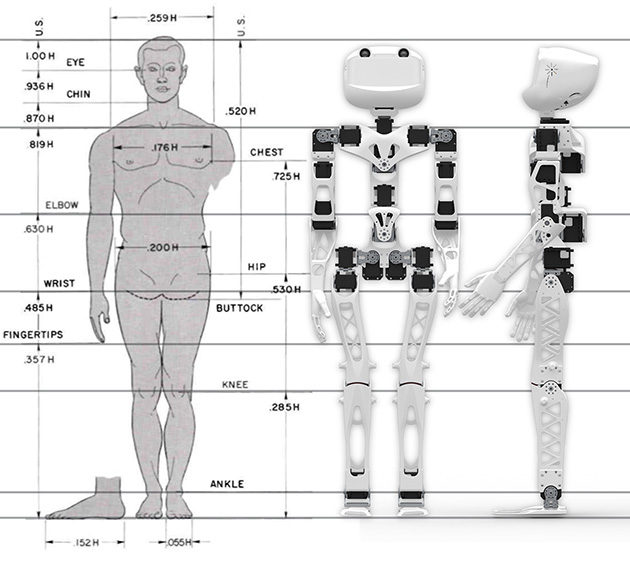
\includegraphics[width=0.8\linewidth]{proportion_poppy.jpg}
    \end{center}
    \caption{Caption here}
    \label{fig:figure1}
\end{figure}


\subsection{Feet} % (fold)

Most of humanoid robots have big feet flat and rectangular feet. This design is indeed really convenient to simplify balance problem while it permits to increasses easily the sustentation polygon.
But this design choice implies some constraints:

First, increasing the foot length inscreasses the lever arm applied to the ankle. It can be useful as it extend the impact of the ankle control over the whole body. Yet given the potential high-torque applied to the ankle, acheiving such control requires very powerful actuator.
However powerful actuators are heavier and therefore the whole actuation design of the robot needs to be powerful in order to be able to make the foot move. Also, considering the inertia, current work on bipedal dynamic balancing seems required leg with no mass to be acheived. Therefore, either the mass of the robot shoudl increass to the mass of leg is negligeable or we should design more lightweight legs.

Secondly, if we look at the nature of legged locomotion, mostly animals have very small feet compare to their overall size, and actually more feet are smalls more the animal seems agile.

For these reasons, even if it appears clearly more simple right now to achieve robot biped locomotion and balancing with big feet, we decided to explore small and lightweight feet.

Petman has small foot and is by far, the most agile biped robot.


flexible feet bruneau2001dynamic
\begin{figure}[tb]
\centering
    \subfloat[][]{\label{fig:frontal_trunk}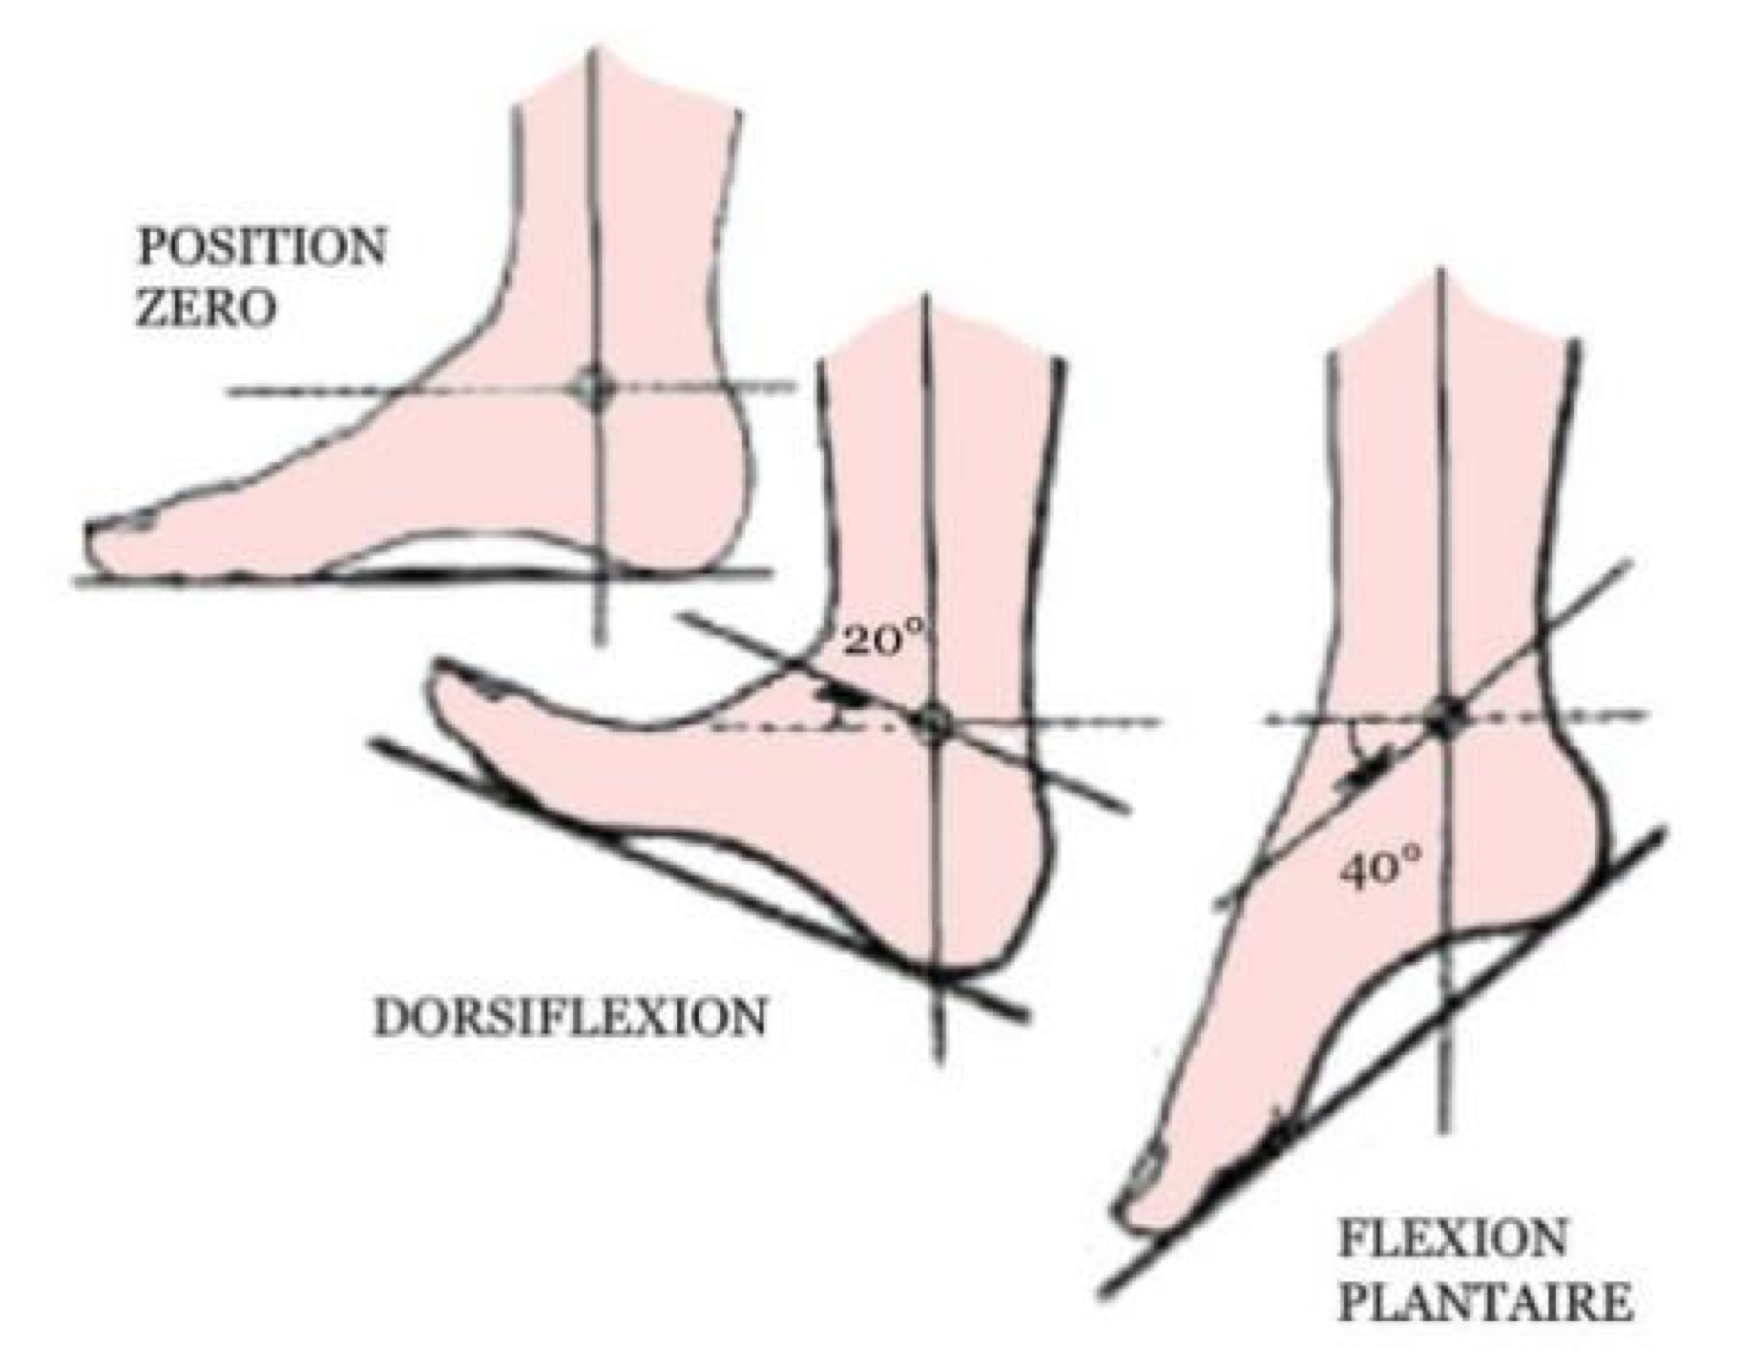
\includegraphics[height=4cm]{human_foot_sagittal.png}}
    \hfil
    \subfloat[][]{\label{fig:sagittal_trunk}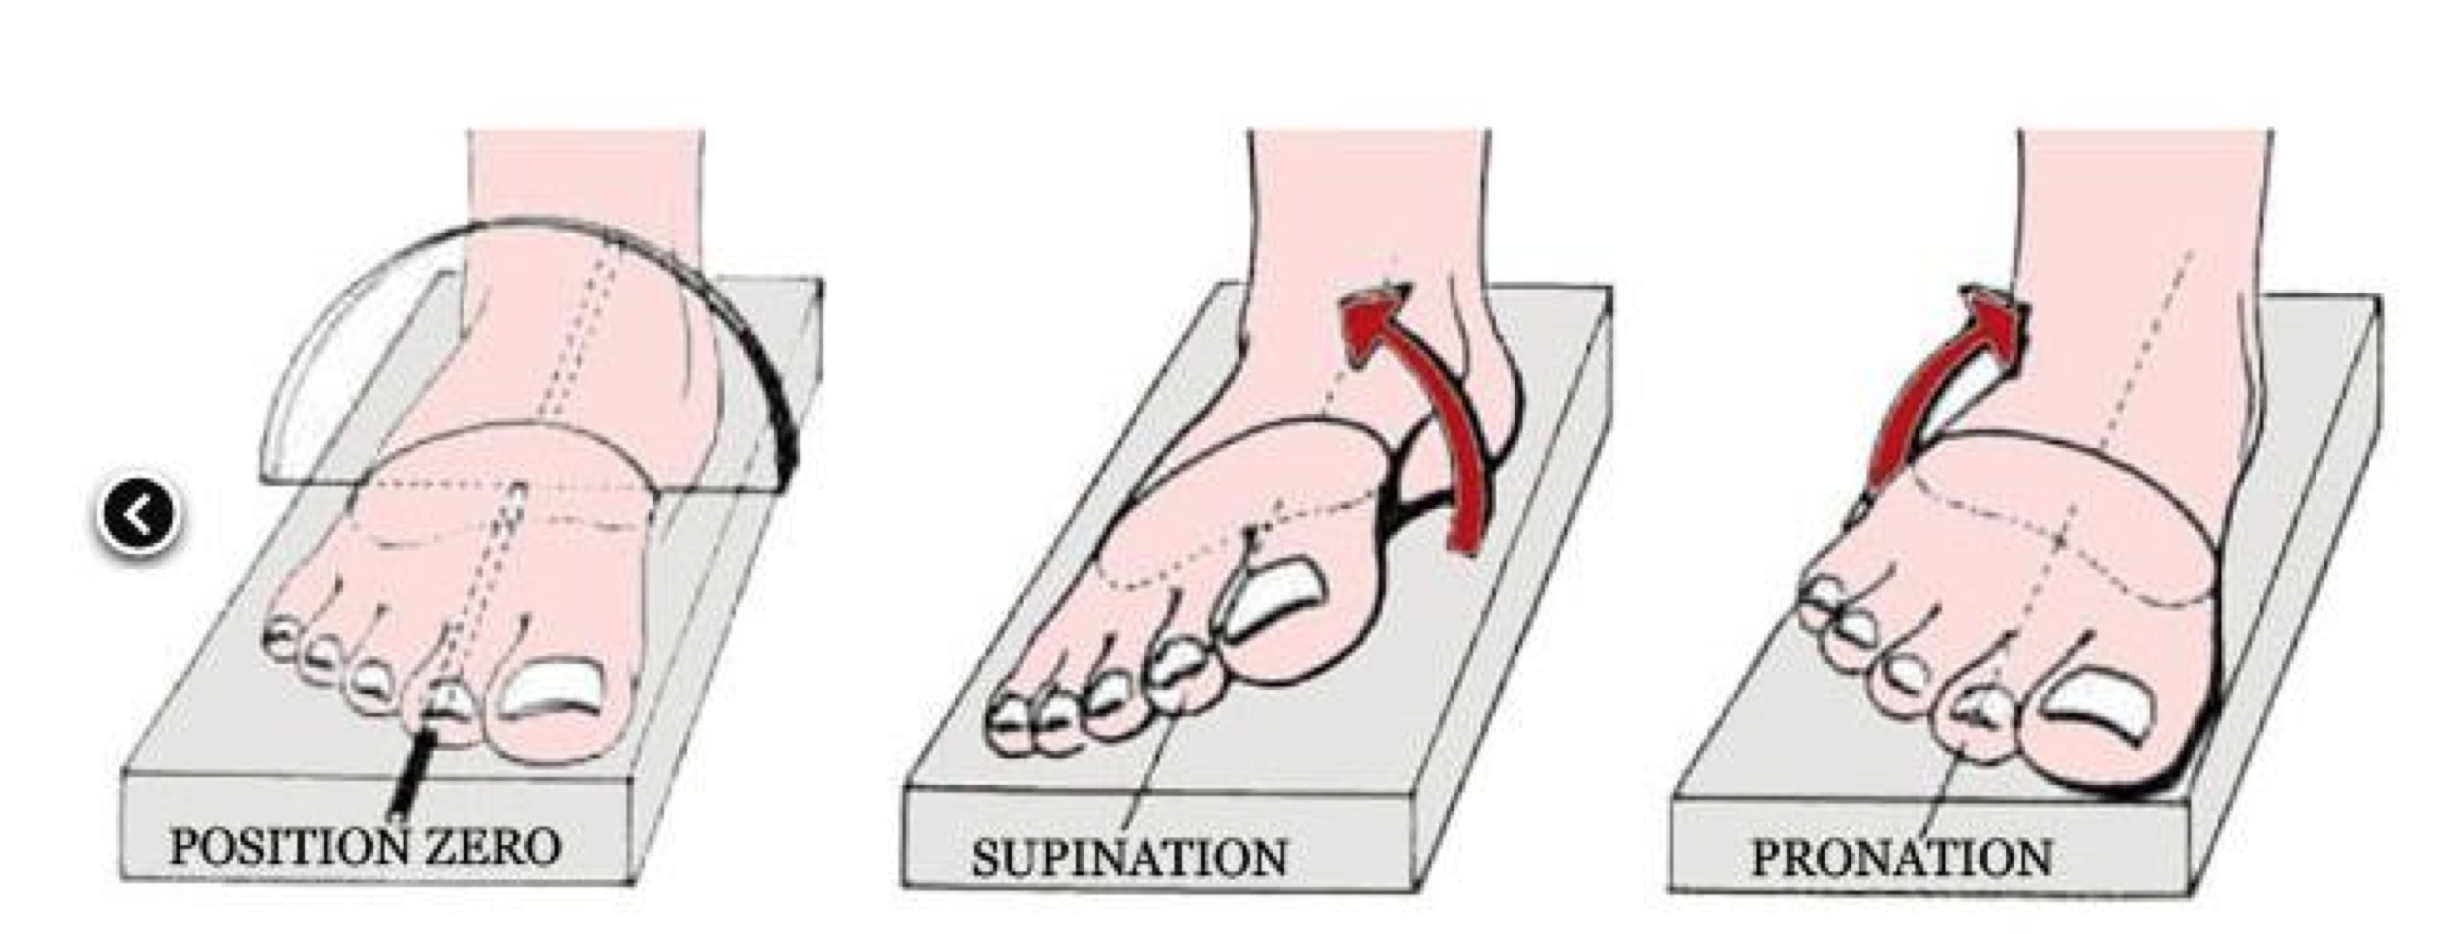
\includegraphics[height=3cm]{human_foot_lateral.png}}
    \caption{}
    \label{fig:poppy_torso}
\end{figure}





Poppy has small foot compare to its height (about 17\%), For example Nao's feet represents 25\% of its height.

Also unlike most humanoids, Poppy only has one active DoF. Indeed, while Poppy has small feet, it appears the actual moment it can transmit to the ground is really little for the lateral motion. Also creating an active articulation would add a lot of mass (72 gr) for little actual effect. Yet this DoF is useful for ground adaptation. We therefore choose to use a passive joint with spring.

\begin{table}[h]
\centering
\begin{tabular}{l| c c c c c}
    & Human & Nao & Darwin Op & Nimbro-OP & Poppy \\
    \hline
    height (cm) & 15 & 25 & 23 & 20 & 83\\
    Foot length (cm) & 15 & 25 & 23 & 20 & 14.5\\
    ratio (\%) & 15 & 25 & 23 & 20 & 17\\
\end{tabular}
\caption{}
\label{tab:poppy_feet_compare}
\end{table}


\begin{figure}[tb]
    \begin{center}
        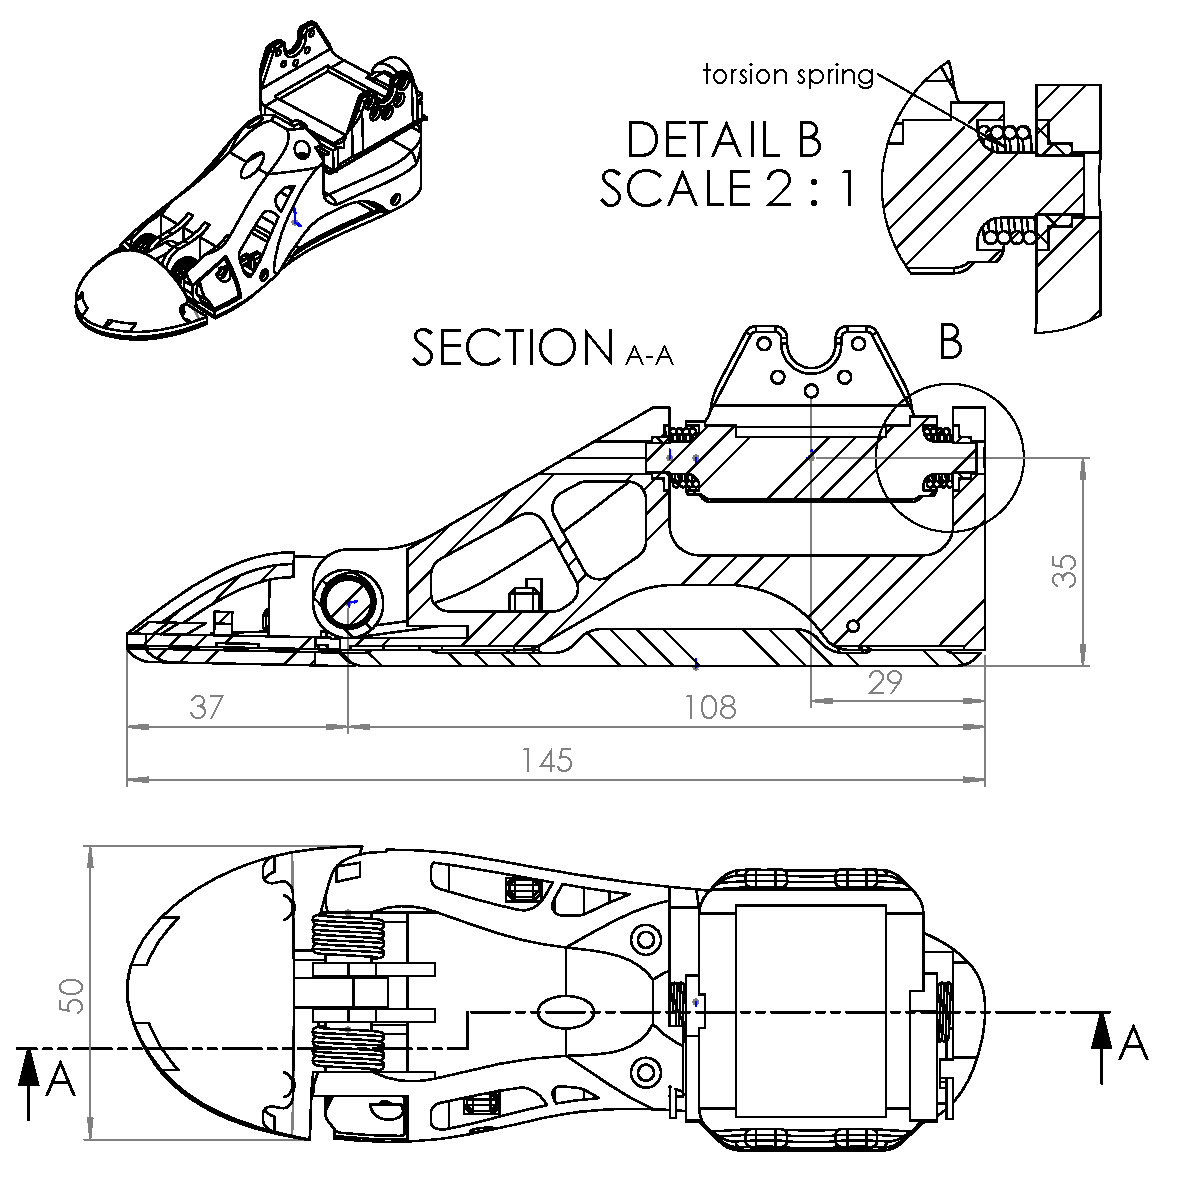
\includegraphics[width=\linewidth]{poppy_foot_v1.pdf}
    \end{center}
    \caption{Caption here}
    \label{fig:poppy-foot-v1-design}
\end{figure}


This design choice as a strong impact on the overall design, because we have lightweight feet, the power requirer to make the leg move is reduced, we can therefore use smaller motors which are also lighter.


\subsection{Legs} % (fold)



If we look closely at the human morphology of the femur, it appears that it is inclined of 6 degrees. This makes the feet closer to the projection of the center of gravity (see Fig.~\ref{fig:human_thigh}.a). We reproduced this on Poppy. While we could have inclined the whole leg, we chose to only incline the upper part of the leg to make all the motors of the leg actuate in the same plane. Both approaches lead to the same two main stability enhancements during walking gait:



\begin{figure}[p]
    \begin{center}
        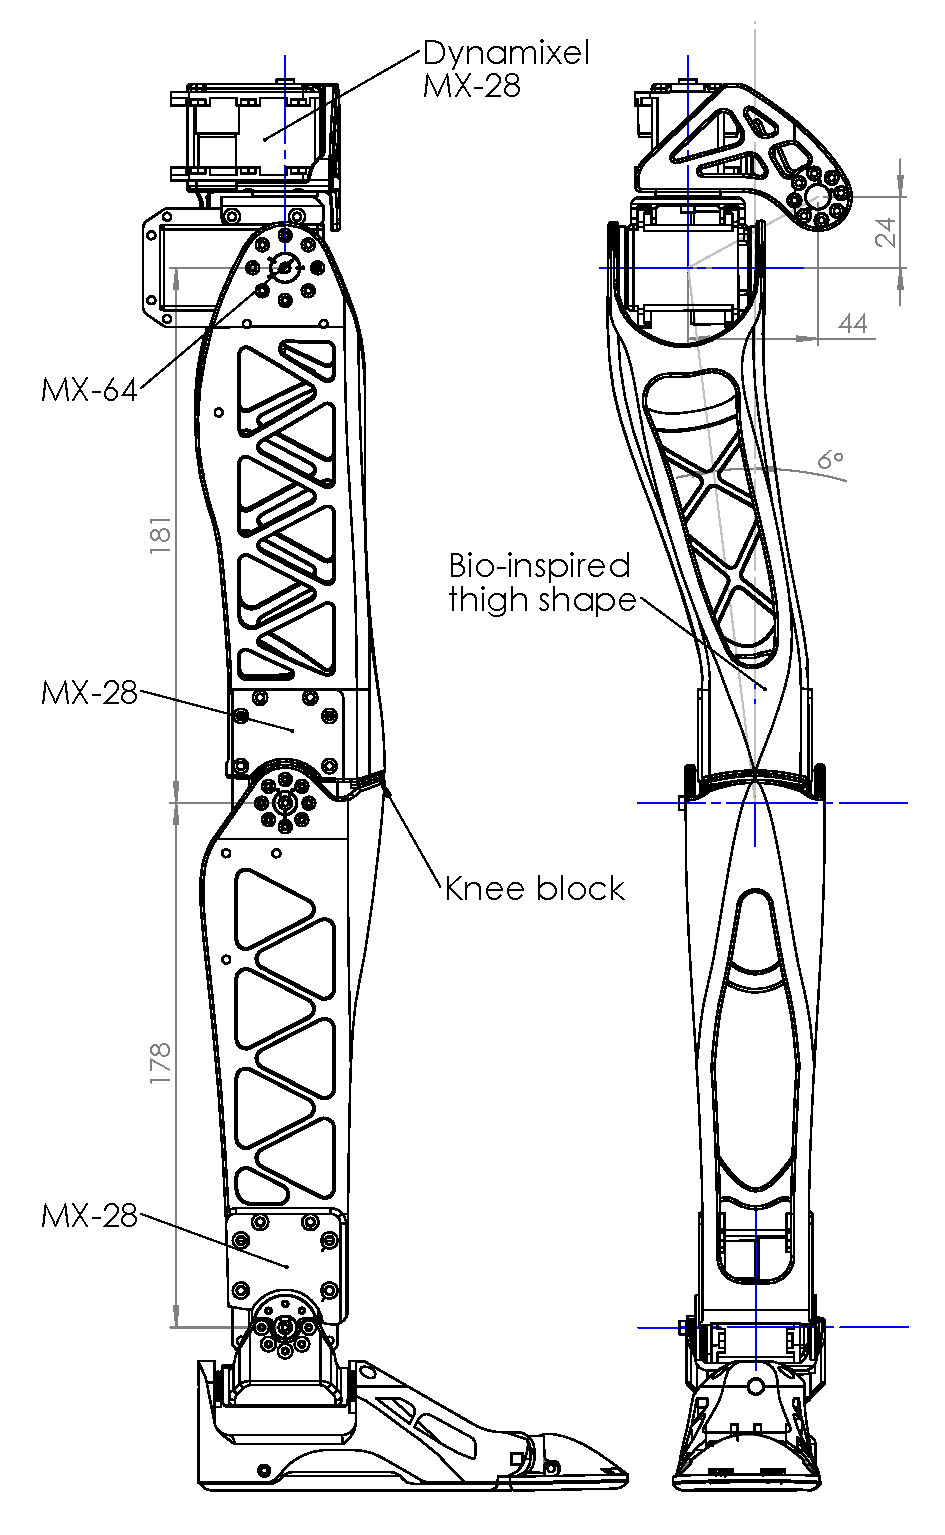
\includegraphics[width=\linewidth]{poppy_leg_design.pdf}
    \end{center}
    \caption{Caption here}
    \label{fig:figure1}
\end{figure}


% subsection feet (end)


% \subsection{Legs} % (fold)


% \subsection{Thigh} % (fold)
% \label{sub:thigh}

% If we look closely at the human morphology of the femur, it appears that it is inclined of 6 degrees. This makes the feet closer to the projection of the center of gravity (see Fig.~\ref{fig:human_thigh}.a). We reproduced this on Poppy. While we could have inclined the whole leg, we chose to only incline the upper part of the leg to make all the motors of the leg actuate in the same plane. Both approaches lead to the same two main stability enhancements during walking gait:

% \begin{figure}[thpb]
%     \centering
%     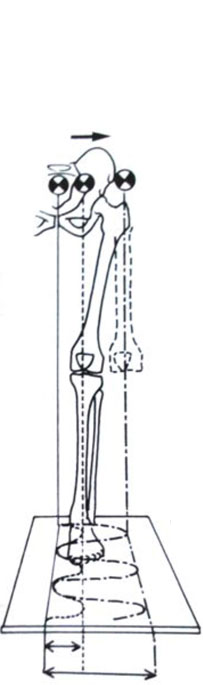
\includegraphics[height=5cm]{human_thigh.pdf}
%     \caption{\emph{left:} Human leg anatomy and effect of the bending femur on the CoG motion during walking gait. \emph{right:} Model for the dynamic comparison.}
%     \label{fig:human_thigh}
% \end{figure}






\section{Hip} % (fold)
\label{sec:hip}


Poppy's small feet increase the challenge of the balance of the robot. Also, to keep the projection of the center of gravity (CoG) inside the support polygon, defined by the feet geometry, it is necessary to control the weight distribution of the robot structure. In particular, we wanted that in its initial upright posture, Poppy stays balanced without any control.

Robotis actuators are among the densest elements in the Poppy platform ($ 1700 kg.m^{3} $) and are the main source of weight ($1.8 kg$). Their spatial distribution represents therefore the major part of the distribution of masses in Poppy. In order to limit the displacement of the mass on the back of the robot, we decided to avoid conventional ball joint assembly for the hip joint such that it is made on most robots based on Robotis motors (i.e. distributed in a plane parallel to the sagittal plane). Instead, we placed them on the frontal plane as the from left to right stability is greater than the from rear to front stability. By doing so, the hip joint is not a real ball joint anymore. Yet, the lost freedom is not relevant for the walking gait.


With this constraint, there are two main solutions for the motor repartition (see Fig.~\ref{fig:hip_choice}a and \ref{fig:hip_choice}b). We chose the second one (b) for the four following reasons:

\begin{itemize}
    \item It is more compact and closer to the human proportion.
    \item Hip rotations (in frontal plane) lead to slight vertical motions of the leg which act as a damper during walking. This damping can be tuned by adjusting the stiffness of the actuator.
    \item It reduces the hip joint lever arm and thus reduces the torque required to maintain position in single support phase.
\end{itemize}


\begin{figure}[p]
    \begin{center}
        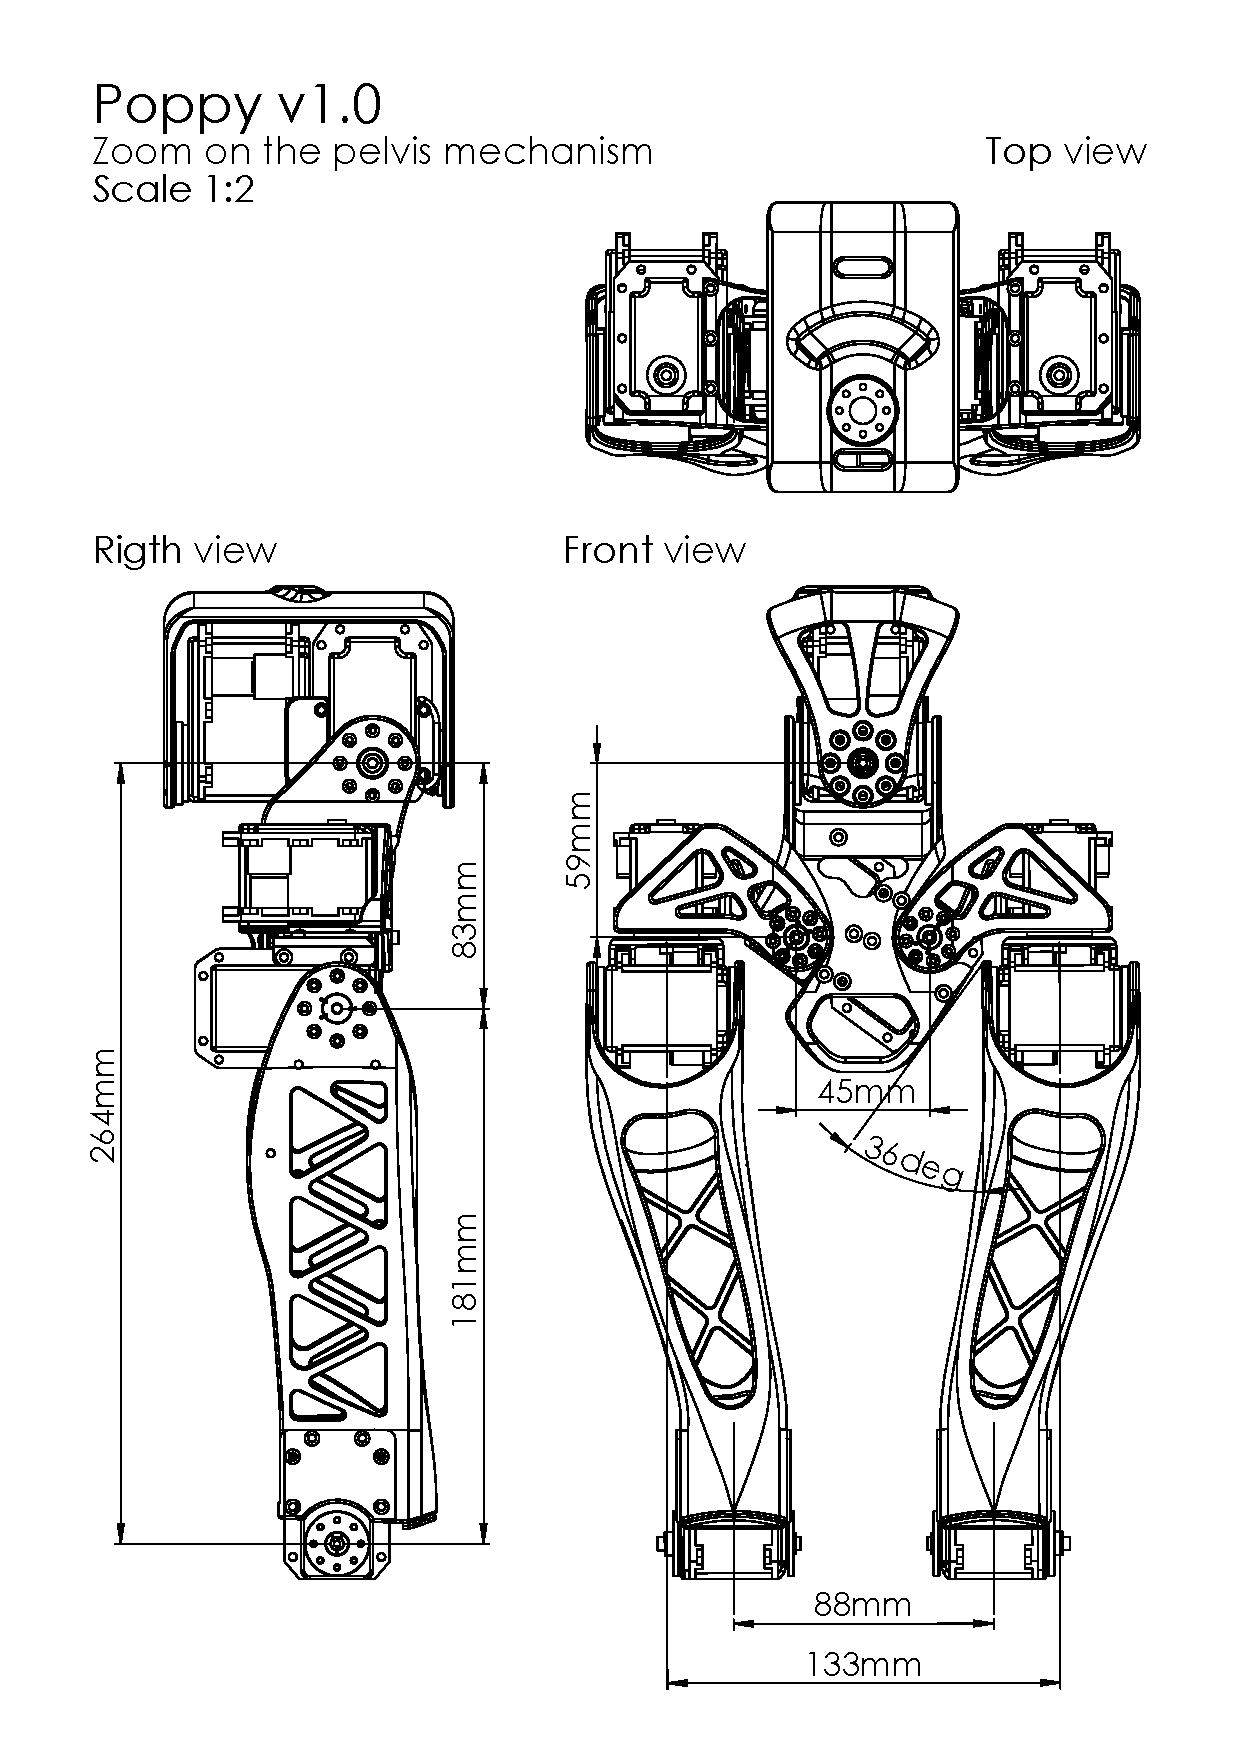
\includegraphics[width=\linewidth]{poppy_zoom_hip_blueprint.pdf}
    \end{center}
    \caption{Caption here}
    \label{fig:figure1}
\end{figure}


% section hip (end)


\section{Multi-articulated torso} % (fold)

Humanoid robots mostly have a rigid torso without any joint (e.g DarwinOp, Nao, NimbroOP) or few DoF (e.g. two for Icub, one for HRP-2).

However if we look the human trunk and in particulat the spine, it has a complex mechanical structure and a large network of dense muscles controlling a very large number of DoFs. It allows for complex motions in several direction while keeping the balance. Its movements are regulated by a complex combination of anticipatory and reactive muscle actions.

Before 1982 and the work of Thorstensson (58), few scientists have really approached the subject. Since, several studies have investigated the activity of the trunk during walking, and showed that the trunk is not only an additional mass but for example participates actively in the walking of Human.
Electromyographics studies showed the importance of the erector spinae muscles in the organization of motor pattern during walking (61),(62),(63) but also of other rhythmic tasks (62). Like the salamander (8), a sequential activation of erector spinae muscles was found (64),(62).
They also show that the trunk is leaning forward and oscillates from 1.5 to 6 deg during walking. In addition, lateral flexion during a gait cycle in the frontal plane promotes the weight shift and opposite rotations of the lumbar and thoracic belts in the horizontal plane allows extend the footstep (59); (60).

Thus the trunk of the human is complex and seems to play an important role in the walking of human, essential to all human movements and especially for walking. The movements of the spine can facilitate the transfer of weight from one leg to the other, improve the balance but also participate in the dynamics of the walking.

It seems therefore interesting to enable a humanoid robot trying to explore the role of morphology, to have an articulated trunk in order to evaluate its impact on several task from dynamic walking to physical human-robot interaction. Yet the human trunk is difficult to replicate on a small robot using servo motors and therefore a simplification is needed.

\begin{figure}[tb]
    \begin{center}
        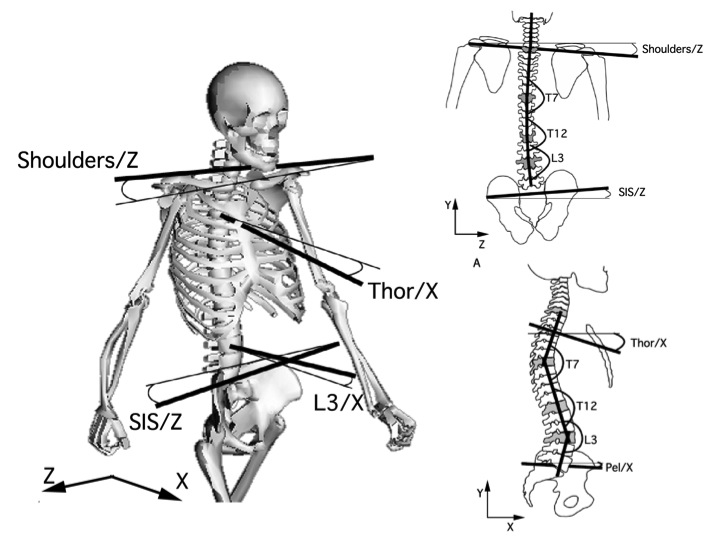
\includegraphics[width=\linewidth]{human_trunk.jpg}
    \end{center}
    \caption{Caption here}
    \label{fig:figure1}
\end{figure}

Interestingly, Ceccato~\cite{ceccatoPlos09} studied the role of trunk during walking and highlighted that there are some places in the spine where the displacements are the most important, i.e. that the apparent high dimensionality of the trunk could be factorized down to a few essential components/dimensions.

Accordingly, it appears we can replicate the essential degrees of freedom of human trunk with two DoFs in the sagittal plane, two in the coronal plane, placed in the pelvis and shoulder /thoracic and one in the horizontal plane placed in the middle of his trunk.

These main degree of freedom have been first introduced on Acroban~\cite{Ly2011bio} and continued on Poppy (see \figurename~\ref{fig:poppy_torso}).

Contrary to the design of the hips, it was not possible here to fit the 5 motors in the frontal plane due to the limited space in the trunk. So to reduce the shifting of the center of gravity to the back of the robot we gradually shifted the upper body to the front. By doing so, we keep the CoG in the support polygon.



\begin{figure}[p]
\centering
    \subfloat[][]{\label{fig:torso_blueprint}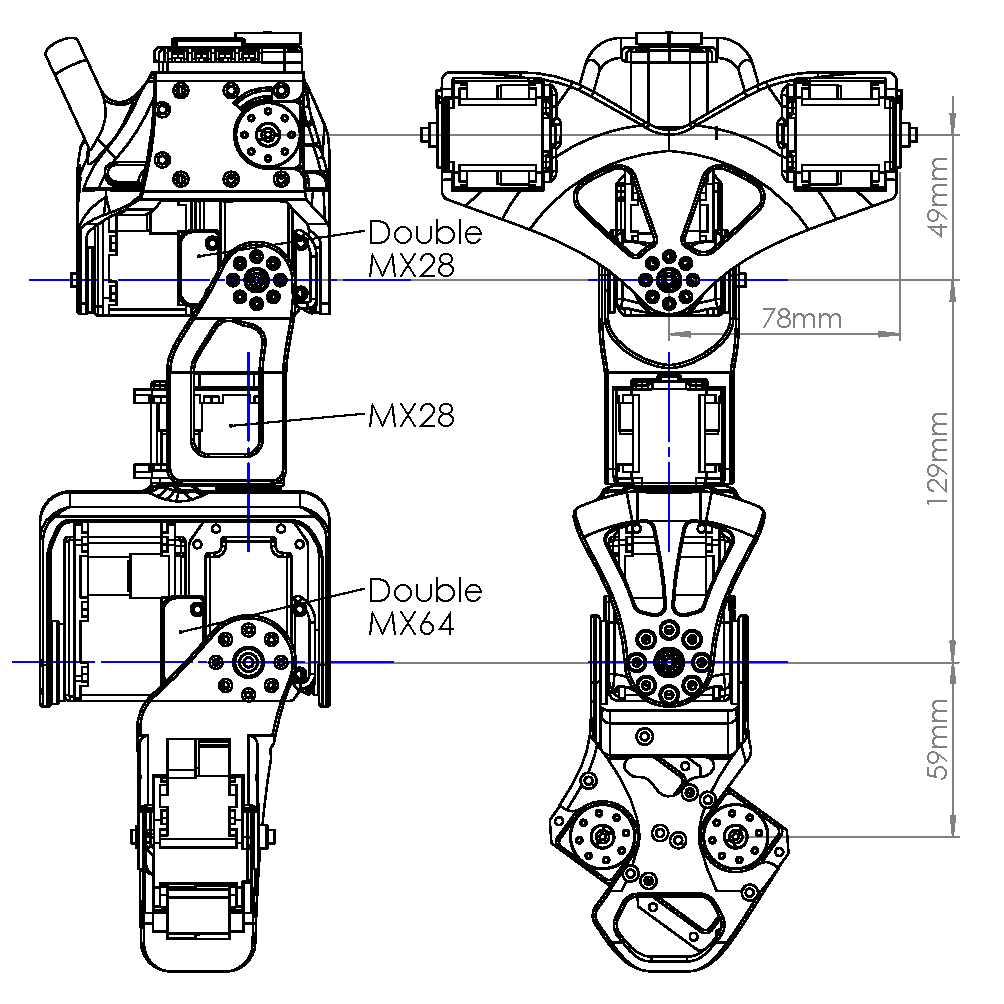
\includegraphics[width=\linewidth]{poppy_torso.pdf}}


    \subfloat[][]{\label{fig:frontal_trunk}\includegraphics[width=0.5\linewidth]{trunk_face.png}}
    \hfil
    \subfloat[][]{\label{fig:sagittal_trunk}\includegraphics[width=0.5\linewidth]{trunk_sagittal.png}}
    \caption{These figures illustrate some morphological features of the Poppy humanoid Robot:\newline a) The Poppy's limbs follow the human being proportion as described in~\cite{dufour2005biomecanique}.\newline b) and c) Poppy has an articulated trunk of 5 DoFs which allows more natural and fluid motions while improving the user experience during physical interaction and actively participating to the balance of the robot.}
    \label{fig:poppy_torso}
\end{figure}




\subsection{Upper limbs} % (fold)

Poppy's arms were not designed for explore grasping but rather for balancing, expressive and interaction purposes. Thus they only involve the minimum articulations to produce a wide range of motion but they do not involve articulated hands.


Thanks to its multi-articulated structure and its expressive head, Poppy has a particularly high potential for creating and studying emotions and gesture social communication (see \figurename~\ref{fig:TER_cognitic}).


% \begin{figure}[tb]
%     \begin{center}
%         \includegraphics[width=\linewidth]{arm_block.png}
%     \end{center}
%     \caption{Caption here}
%     \label{fig:figure1}
% \end{figure}


\section{Conclusion} % (fold)
The first fonctionnal version took 4 months to be built


\section{Discussion} % (fold)



% \chapter{Poppy} % (fold)

% \section{poppy's size}


%


% \subsection{The size} % (fold)
% The basic version of Poppy is about 80cm height.

% More the robot is tall, more is it interesting to explore the morphology role. Indeed, when link length is increasing we can no longer ignore dynamic and inertia.

%  It represents a compromise between a really transportable robot but long enough to explore dynamic properties. With such long leg, it is necessary to use the


% In order to develop an adapted mechanical structure, we interested ourselves in how evolution solved sensorimotor task related to locomotion and in particular bipedal locomotion. As human locomotion represents one of the finest example of mastering bipedal walking, we took functional inspiration of some elements that seem relevant to improve the locomotion of humanoid robots.

% \begin{figure}[thpb]
%     \centering
%     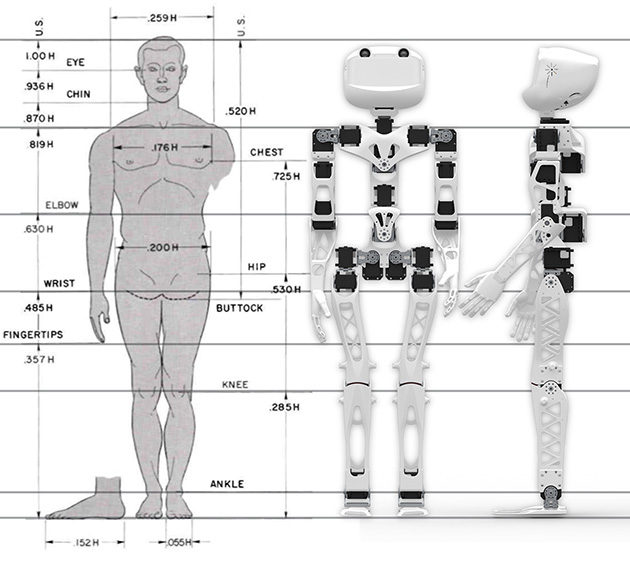
\includegraphics[width=6cm]{proportion_poppy.jpg}
%     \caption{Human proportion used for the design of Poppy \cite{dufour2005biomecanique}}
%     \label{fig:proportion_poppy}
% \end{figure}

% This bio-inspiration is expressed on the whole structure of Poppy. On the anatomical point of view, it reproduces the human proportions as described in the literature \cite{dufour2005biomecanique}  (see Fig.~\ref{fig:proportion_poppy}) and their sensorimotor space organization: i.e. the main degrees of freedom (actuated and passive), an inertial unit in the head and force sensors distributed underfoot.

% As explained in \ref{sec:introduction}, biped locomotion is a central design goal of the Poppy platform. For this purpose, the morphological optimization is mainly expressed on the locomotive system (legs and trunks) in order to increase the robot robustness, agility and stability during the walking.
